\documentclass{article}

\usepackage[margin=1in]{geometry} 
\usepackage[english]{babel}
\usepackage[T1]{fontenc}
\usepackage[utf8]{inputenc}
\usepackage{amsmath,amsthm,amssymb,amsfonts, fancyhdr, color, comment, graphicx, environ}
\usepackage{xcolor}
\usepackage{mdframed}
\usepackage[shortlabels]{enumitem}
\usepackage{indentfirst}
\usepackage{hyperref}
\usepackage{lastpage}
\usepackage{listingsutf8}
%\usepackage{ff++listings}
\usepackage{amsmath}
\DeclareMathOperator{\Tr}{Tr}

\usepackage{physics}
\usepackage{amsfonts}
\usepackage{float}
\PassOptionsToPackage{hyphens}{url}\usepackage{hyperref}

\newenvironment*{remerciements}{%
\renewcommand*{\abstractname}{Acknowledgements}
\begin{abstract}
}{\end{abstract}}

\usepackage{xurl}

\renewcommand{\footrulewidth}{0.8pt}
\hypersetup{
    colorlinks=true,
    linkcolor=blue,
    filecolor=magenta,      
    urlcolor=blue,
}

\pagestyle{fancy}

\newenvironment{problem}[2][Etape]
    { \begin{mdframed}[backgroundcolor=gray!20] \textbf{#1 #2} \\}
    {  \end{mdframed}}

\newenvironment{solution}{\textbf{Réponse}}

\lhead{Florent Pollet}
\rhead{ES2A EEP-02} 
\chead{\textbf{Vaccine strategies}}
\lfoot{Véronique Stoven}
\cfoot{Mines Paris}
\rfoot{\thepage/\pageref*{LastPage}}


\let\up\textsuperscript

\usepackage{biblatex}
\addbibresource{biblio/biblio.bib}

%\usepackage[backend=bibtex]{biblatex}
\usepackage[nottoc, notlof, notlot]{tocbibind}

\begin{document}

    \title{\Large ES2A EEP-02  \\[0.5cm]
        \bf\Large Vaccine strategies}
\author{\large Florent Pollet \ \\}
\date{\large\today}

\makeatletter
    \begin{titlepage}
        \begin{center}
	   { 
\includegraphics[width=12cm]{imgs/mp_logo.png}}
	   {\ \\ \ \\}
        \vbox{}\vspace{2cm}
            {\@title }\\[1cm] 
            %{ \includegraphics[width=7cm]{imgs/cover.PNG}}\\[1cm]
            {\@author}

            {\large \ \\ Supervisor: \bf Véronique Stoven\\ \ \\}
            {\@date\\}

        \end{center}

        \vspace{4cm}
        \begin{figure}[H]
            \centering
            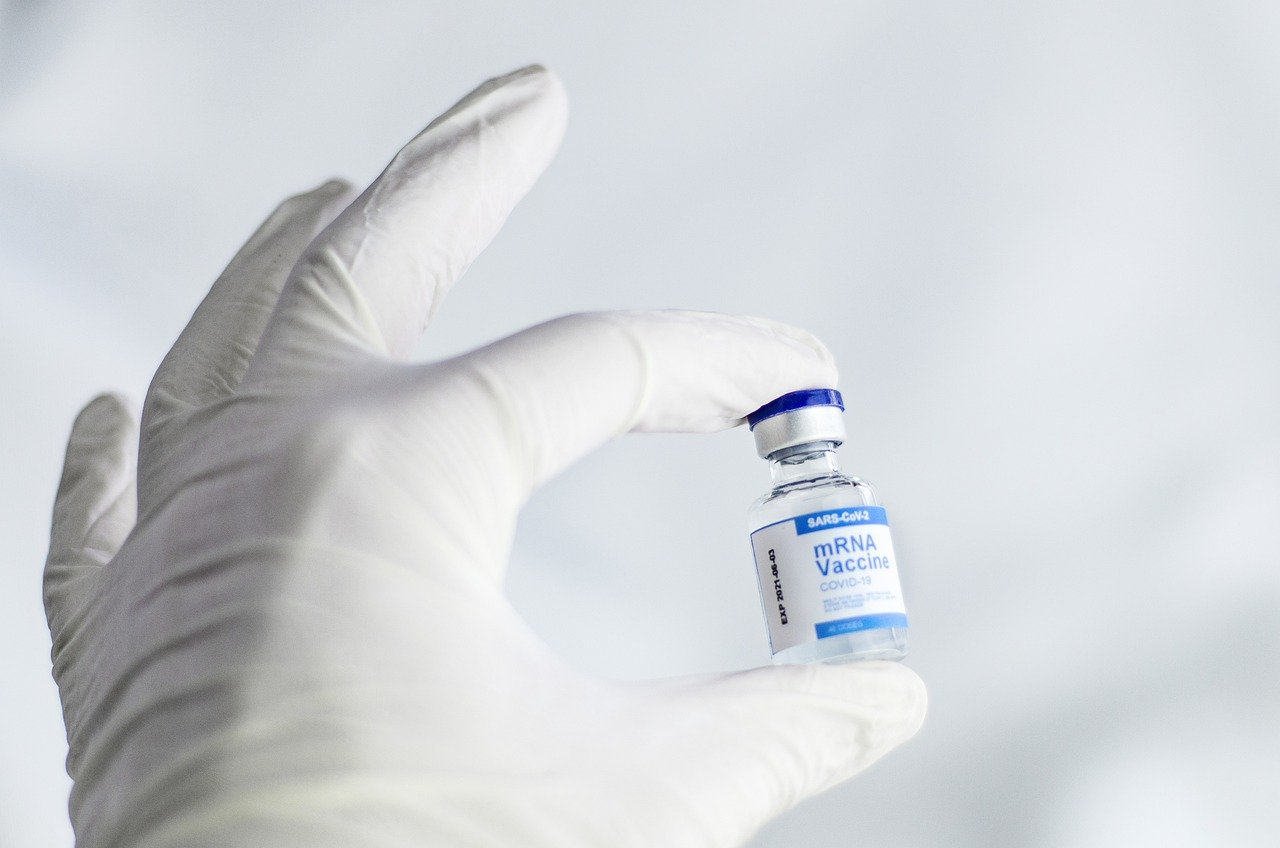
\includegraphics[width=0.4\textwidth]{imgs/vaccineCover.jpg}
        \end{figure}

    \end{titlepage}


    \begin{abstract}        
        In a context of a pandemic and major doubts towards vaccination among populations, this paper deals with vaccine strategies, especially how mRNA vaccines are revolutionizing them.
        It is clear that immunology represents a complex field of science,
            and nowadays the breakthroughs in biotechnologies are offering new possibilities to accelerate vaccine development, efficiency and safety as well as a better understanding
            our immune system.
        This paper aims at summarizing the different vaccine techniques with a special attention to mRNA vaccines\footnote{Messenger RiboNucleic Acid}, in order to
            have an overview of the current vaccine strategies which are going to evolve.
        % implications, finding, methods ? go further ?
    \end{abstract}

        
    \begin{remerciements}
        I cannot express enough thanks to my teacher Véronique Stoven for her interesting lessons about molecular and synthetic biology,
            which inspired me this topic.
        I absolutely loved doing research and writing this report.
    \end{remerciements}


    \tableofcontents


    \newpage

    \makeatother

    \section{Introduction}

    Vaccines represent an amazing invention which saved millions of lives in the world since 2000 \autocite{HowManyLives2021}.
    Even if vaccination is not new, the recent pandemic of COVID-19 brought to the forefront this field, generating great advances but also important debates about safety, ethics and politics.
    It is necessary to take into account all these changes and to adapt to be avoid a backward step and the rejection of these opportunities. 
    
    Therefore it would be interesting to better understand the recent evolutions in vaccine strategies and technologies and the consequences it may have on society.
    
    Firstly, I will briefly recall the history of vaccination, detailing the different types of vaccines which have been developed.
    Secondly, I will present the technology of mRNA (messenger ribonucleic acid) vaccines which are currently the main source of progress.
    Thirdly, I will observe how society is integrating these developments and what issues remain to be solved.

    This theme is closely linked to the mechanics of the immune system, in medicine, which will not be detailed in this article due to the needed knowledge in medicine.
    In any case, I would like to thank Ms. Stoven for her molecular biology course and her help in the writing of this article.

    \section{A brief history of vaccines}

        \subsection{Discovery of the principle}

            The principle of vaccination could come from the idea of mithridatism, that is to say the ability to gain protection against a poison by taking several benign amounts.
            
            Variolization, which corresponds to injecting smallpox pustules to gain immunity against smallpox, began in China around the 10\up{th} century \autocite{canouiHistoryPrinciplesVaccination2019}. 
            Before the scientist Jenner, several persons realized variolization in England. However, in 1798, this is Jenner who made a link between cowpox and smallpox: 
                cowpox could an attenuated version of smallpox.            

            The idea of vaccination is to create an individual, long-term and efficient protection against a pathogen (like a virus or a bacteria), without causing serious symptoms.
            This is made possible thanks to the memory of human's immune system.

            The word "vaccination" comes from the Latin word "vacca", which means "cow".

            \subsubsection*{The immune system at a glance}

                In the medical field, the immune system is mainly composed of two parts:

                \begin{itemize}
                    \item The innate immune system. After the infection, it is the first system to react. It is mainly represented by Natural Killers (NK) cells,
                            phagocytes and dentritric cells which play an important role to initiate the adaptive response\footnote{The details for each different type 
                                of cells will not be covered in this report.}.
                    \item The adaptive (or acquired) immune system. This one is subdivised in two categories: 
                        \begin{itemize}
                            \item The cellular response, thanks to lymphocytes T (thymus) CD8+ (cluster of designation). They are cytotoxic and they can kill the infected cells.
                                    To be efficient, in most cases, they need the major histocompatibility complex.
                            \item The humoral response, thanks to lymphocytes B (Bursa of Fabricius). They produce antibodies (immunoglobulines, abbreviated Ig), which are proteins able to 
                                    neutralize microbial effectors, from bacteria and viruses. Antibodies need antigens of the pathogens, which are proteins expressed by the pathogen, to recognize them.
                        \end{itemize}
                        Lymphocytes T CD4+ (helper) regulate both responses.
                        The specifity of the adaptive immune system is its memory thanks to specific T and B memory cells, 
                            and it can be easily observed using the concentration of immunoglobulines in the blood.
                        
                            \begin{figure}
                                \centering
                                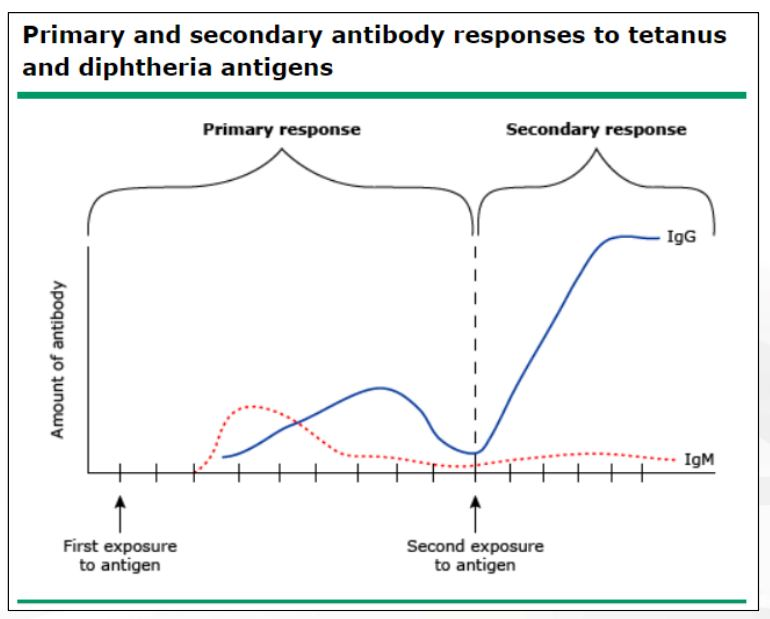
\includegraphics[width=0.5\textwidth]{imgs/PrimarySecondaryResponses.JPG}
                                \caption{Primary and secondary responses to specific antigens \autocite{pinkComparisonImmunityGeneral}}
                                \label{fig:responses}
                            \end{figure}

                        The graph \ref{fig:responses} shows that the response after the first infection is less important and slower after the second one.
                        It also compares the concentration of IgM, an immoglobuline which are non-specific, 
                            versus IgG, which are more specific microbial effectors such as toxines or proteins:
                            it proves that the adaptive immune system becomes efficient after the innate system, and that there is a memory effect on the second infection.

                        % ANTIBODY, ANTIGEN picture?

                        The cellular response is more complicated to quantify.

                        As regards pathogens, the incubation period can be short (pneumococcus) or long (hepatitis B virus).

                        It is important to notice that the immune system is very different according to the age of the person: the main phenomenon when ageing is immunosenescence,
                            which makes the immune system less reactive and dynamic.
                \end{itemize}
              
        \subsection{First generation of vaccines}
            
            It is only between 1870 and 1885 with Pasteur's works (helped by Emile Roux and Emile Duclaux, and based on Robert Koch's findings), 
                that the first vaccines were developed \autocite{plotkinHistoryVaccination2014}.
            The first official vaccines that he conceived were against chicken cholera, anthrax, swine erysipelas and then rabies.

            The first generation of vaccines consists in pathogens which are live, weakened or killed. Live weakened vaccines are the most immunogenic,
                but they should be prepared carefully. Despite being efficient, there are still high risks using them if virus are not attenuated enough:
                one can develop the disease and transmit it to an immunocompromised person. Otherwise, vaccines can be killed for example with heat/chemical treatment, and they
                are less dangerous, however there is a need for adjuvants (from the Latin word "adjurvare", which means "to help") 
                to make them immunogenic, and the response is mainly humoral and less cellular.

            Adjuvants can be very diverse and numerous as well as their mechanism of action: killed mycobacteria, oils, 
                aluminium salts, microparticles, squalanes, ligands of 
                PRRs... They aim at amplifying the reaction for a whole population and each individual (especially old people whose immune system is less dynamic) and 
                at reducing the quantity of active substance needed (dose sparing). The dosage should be very cautious not to hide the active substance.
                
            To prepare those vaccines, cell culture is often needed. 
            To weaken viruses, other environments than human cells are used such as chicken cells so that the virus is no more adapted to human cells...

            To prepare a live weakened vaccine, the virus or the bacteria is replicated in adverse conditions several times. Main vaccines of this type are BCG
            (Bacillus Calmette-Guérin vaccine, against tuberculosis), the Mumps vaccine. It is important to note that different vaccines can be combined together,
            like with the MMRV vaccine (Mumps, Measles, Rubella and Varicella: a tetravalent vaccine). It is not dangerous for health and avoid too many injections for children,
            who must develop an immunity for many diseases in the first years.            
                       
            %https://www.pnas.org/content/111/34/12283

            Thanks to the development of immunology and microbiology, in particular the ability to isolate pathogens, vaccines were better understood
                and it led to the development of a new type of vaccines.

            The method of production of these vaccines also evolved over time. With genetic engineering and reverse genetics, that is to say,  
                contrary to forward genetic, the ability to know which phenotypes can be controlled by different genetic sequences,
                it allows a better treatment of viruses to select inactivated vaccines.


        \subsection{Second generation of vaccines}

            % https://vaccine-safety-training.org/subunit-vaccines.html

            This generation demands more development and technological advances,
                to use subunits of viruses such as protein antigens or inactivating toxins produced by the pathogen. %recombinant protein components (antigens for instance).
            There is also the need for adjuvant, which are substances which trigger a powerful immune response ; otherwise the vaccine would not be effective. 
            The response is again mainly humoral: sometimes it cannot activate Toll-Like Receptors on dentritic cells needed for a complete response.

            Subunits vaccines (also called acellular vaccines) are stable and safe, with no risk to induce the disease but the right part of the virus should be choosen.
                They can be protein-based, with polysaccharides, which is a sugar capsule produced by some pathogens (however it has less effect than proteins), or both (it is then called conjugate).
            Inactivated toxins are called anatoxin is a toxin which has lost his toxic power thanks to heat and formaldehyde, but not totally its immunogenic ability.

            To produce these units, the pathogen is cultivated at large scale before using chemicals to destroy and separate the parts of the pathogen.

            Lots of recent vaccines use this technique: influenza, hepatitis A, HPV (Human papillomavirus infection), pertussis, tetanus (anatoxin). 
                The first approved subunit was against hepatitis B in 1981 in the United States. 
                At that time, it was a breakthrough because it represented the first vaccine to protect against liver cancer and against a sexually transmitted disease.

        \subsection{Towards a third generation}

            The third generation of vaccines can be described as genetic vaccines, since it is using genetic sequences to support information of the pathogen. 
            It was made possible thanks to the latest discoveries in biotechnologies and genetics such as gene sequencing \autocite{chavdaDNAVaccinesSARSCoV22021}.  

            There are three main categories:
            \begin{itemize}
                \item Viral vector vaccines: a specific gene of the pathogen is put into an innocuous virus for humans. 
                        This harmless virus can deliver the selected genetic material of the pathogen into the human cells.
                        Then the cells produce proteins from the pathogen which can be used to train the immune system as a classic vaccine.
                        For instance, the vaccines from the firm AstraZeneca and the Oxford University or Janssen against Covid-19 rely on this technique.
                        A major drawback of viral vector vaccines is that it also makes us immune against the vector virus, 
                            which in the future will have difficulties to deliver the genetic material.
                \item mRNA vaccines: this will be discussed in the next section.
                \item pDNA (Plasmid DesoxyriboNucleic Acid) vaccines: the gene from the pathogen is encoded with DNA instead of RNA
                    and it is injected in our cell thanks to the same technique as mRNA vaccines.
                    Nevertheless it must be carefully studied because of the possible effects on human DNA.
            \end{itemize}

            % tab récapulatif

    \section{mRNA vaccines: a promising technology}

        \subsection{Principle}

                It is important to understand the differences between \emph{in vitro}, \emph{in vivo} and \emph{in situ}.

                The two first incentive were quicker development (with a financial and medical interest) and a wider and safer immune response.
                However, it can lead to other uses and it creates new perspectives as regards therapies.

                % mRNA as the blueprint for a protein of the pathogen
                % temps de développement

                %nano lipid instead of virus.
                %difficult to store
 
                cf \autocite{maruggiMRNATransformativeTechnology2019}
                % ntrinsic adjuvant properties because of their recognition by specific
%pattern recognition receptors (PRRs) and elicitation of innate immune
%responses, which are critical for maturation of dendritic cells (DCs) to
%enhance the induction of subsequent adaptive immune responses.

        \subsection{Development}

            The first tests were realized in the 1990s by Wolff. \autocite*[]{wolffDirectGeneTransfer1990}
            But much progress has been needed in the 2000s as regards the synthesis of mRNA.

        % Severe acute respiratory syndrome coronavirus 2 (SARS‑CoV‑2)
        % https://www.medpagetoday.com/special-reports/exclusives/91604
        % Upon vaccination, nucleic acid-based vaccines mimic a viral infection to express vaccine antigens in situ, resulting in induction of both humoral and cytotoxic T cell responses.
        % https://www.sciencedirect.com/science/article/pii/S1525001619300413?via%3Dihub

        % eradication of smallpox and polyomyelite

        % ideal vaccine before ARNm possibilities:  alive weakeaned vaccine, injected into the mucous membranes, to stimulate IgA production

        % usual : injection sous-cutanée, intradermique (peau) ou intramusculaire (plus profond), intraveineuse
        %https://www.google.com/url?sa=i&url=https%3A%2F%2Fwww.infirmiers.com%2Fetudiants-en-ifsi%2Fcours%2Fadministration-d-un-vaccin.html&psig=AOvVaw1kw-yPymOdrfp6v5eTiI-n&ust=1643840900387000&source=images&cd=vfe&ved=0CAsQjRxqFwoTCLDcp9nG3_UCFQAAAAAdAAAAABAD
        % empirical choice before understanding that the aim is to choose the best dentritic cells


        \subsection{Advantages and drawbacks}

            Among the technologies of third generation, it is the most promising compared to viral vectors and pDNA vaccines in terms of efficiency.

            The main advantages are:
            \begin{itemize}
                \item It embodies the idea of "vaccine on demand".
            \end{itemize}

            The main drawbacks are:
            \begin{itemize}
                \item It is very difficult to preserve the vaccine because mRNA is not stable.
            \end{itemize}

        % https://www.amazon.fr/Basic-Immunology-Book-Functions-Disorders-ebook/dp/B07N8ZKYPQ?asin=B07N8ZKYPQ&revisionId=4497585a&format=1&depth=1
        
        \begin{center}
            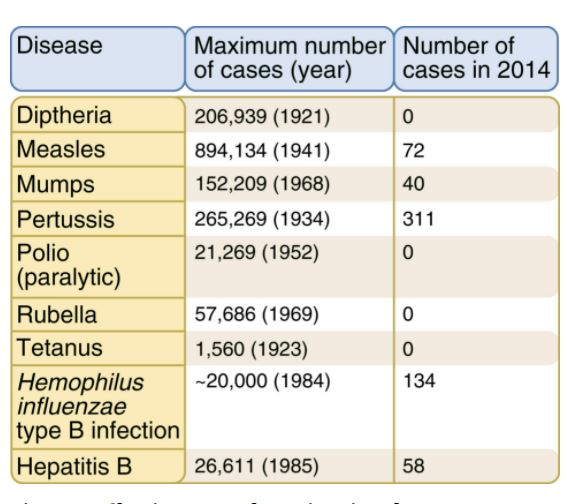
\includegraphics[width=0.5\textwidth]{imgs/NumberOfCases.JPG}
        \end{center}


        % Diphtheria and Poliomyelitis almost disappeared
        % only way to heal some serious diseases

        % drawbacks: anaphylactic shock
        % different according to the types
        % development costs and time

        % side effects: local pain, fever during a few days, fatigue

        % a few people Guillain–Barré syndrome

        
            % majority : humoral response which can be measured to know if something is protected against a disease

    \section{New stakes for vaccines in the 21\up{st} century}

        \subsection{World inequalities}

        % storage constraints
        % WHO: "immunization agenda 2030"; global strategy: to put efforts together, 
        % some regions in Africa more difficult

        % https://www.immunizationagenda2030.org/scorecard for slides and explanations

        
        \begin{center}
            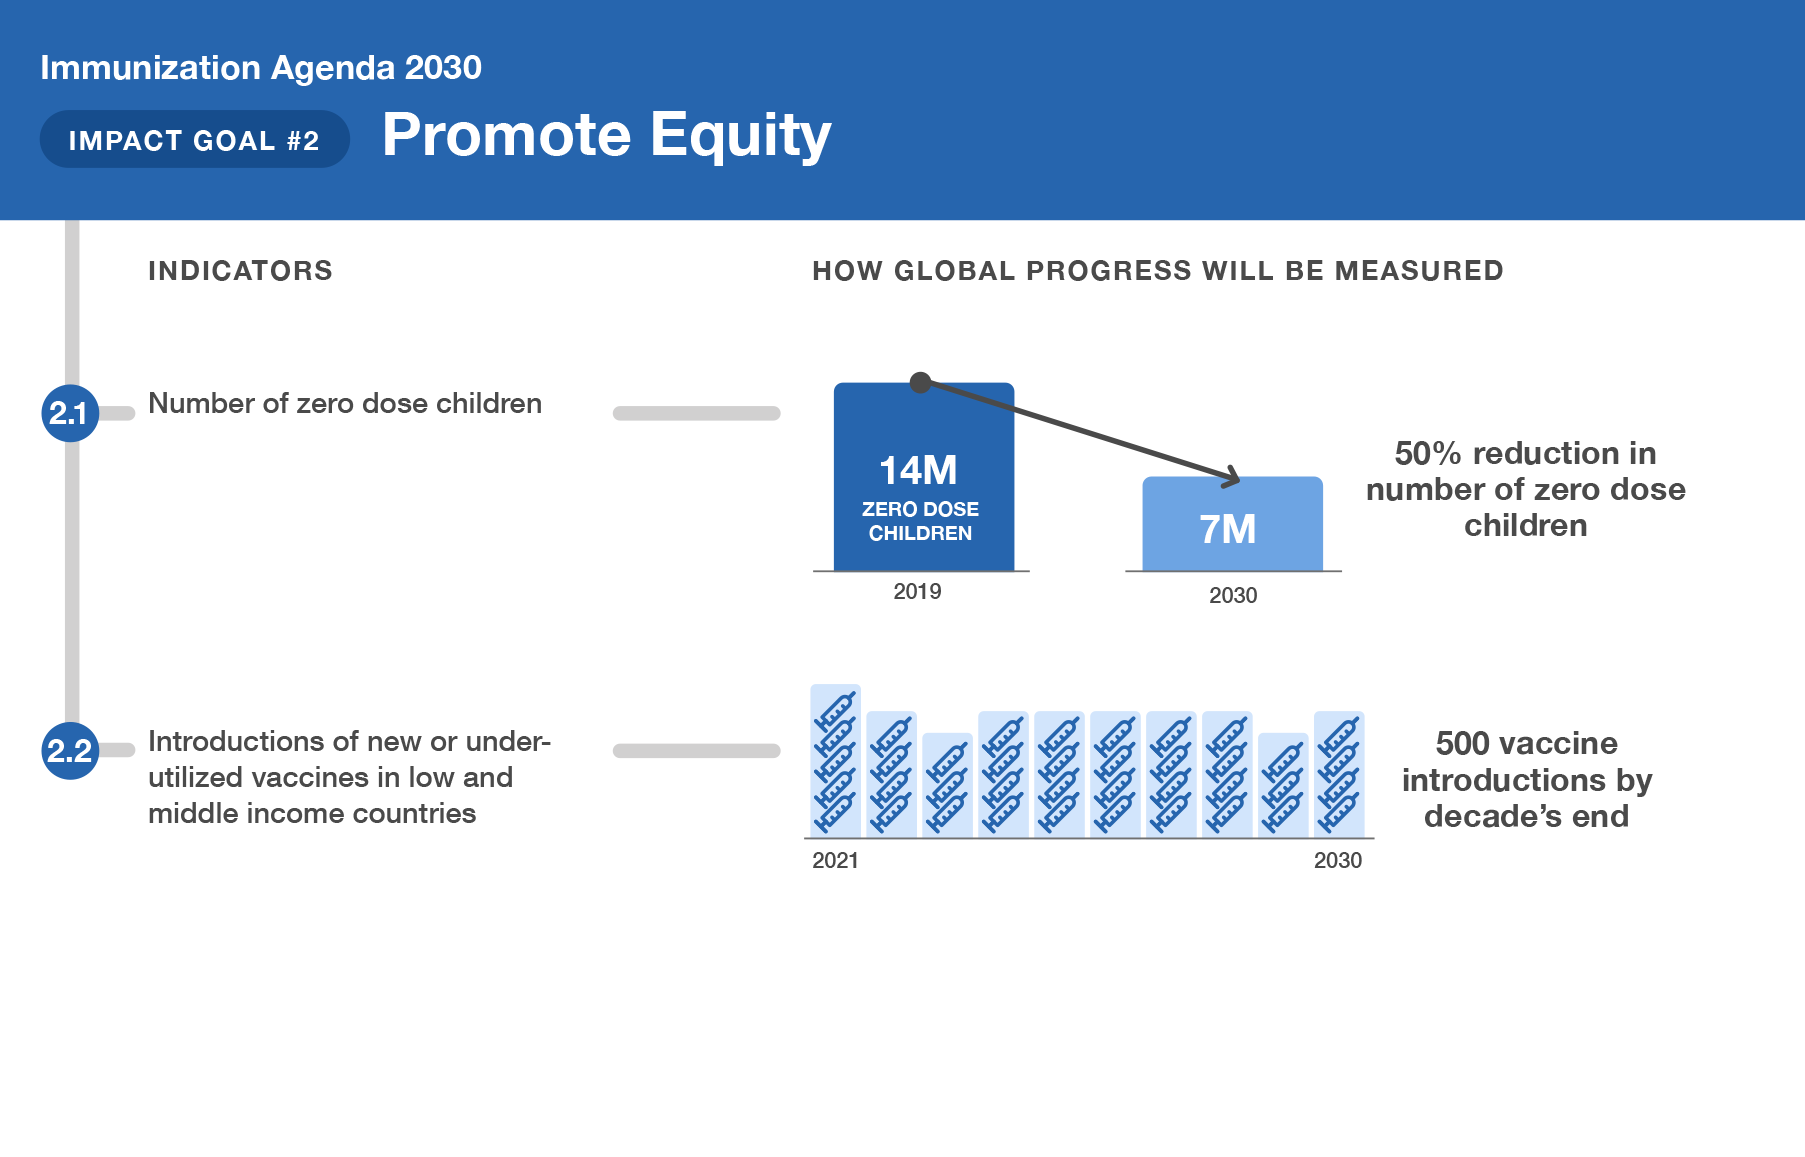
\includegraphics[width=0.5\textwidth]{imgs/IA2030_Scorecard_May23-3.png}
        \end{center}

        \subsection{Public policies}

               % first and second response for a better efficiency : vaccine booster, like for COVID
                % secondary response, a few month after the primary
                % primary response : 15 days min

                % intramuscular, subcutaneous, intradermic or mucosa injection
                

                % deferred protection but durable protection

                % variant: serotherapy, only humoral, passive and temporary, by injecting immunoglobulines

            % variole eradication


            % schéma rappel et courbe antibodies dans les stratégies de vaccin
        % In Frce: vaccine agenda: recommendations & obligations

        % stakes with measles: need high vaccine coverage to avoid outbreaks

        % vaccines for travelling + professionnal

        % perception of side effects, controversies
        \begin{center}
            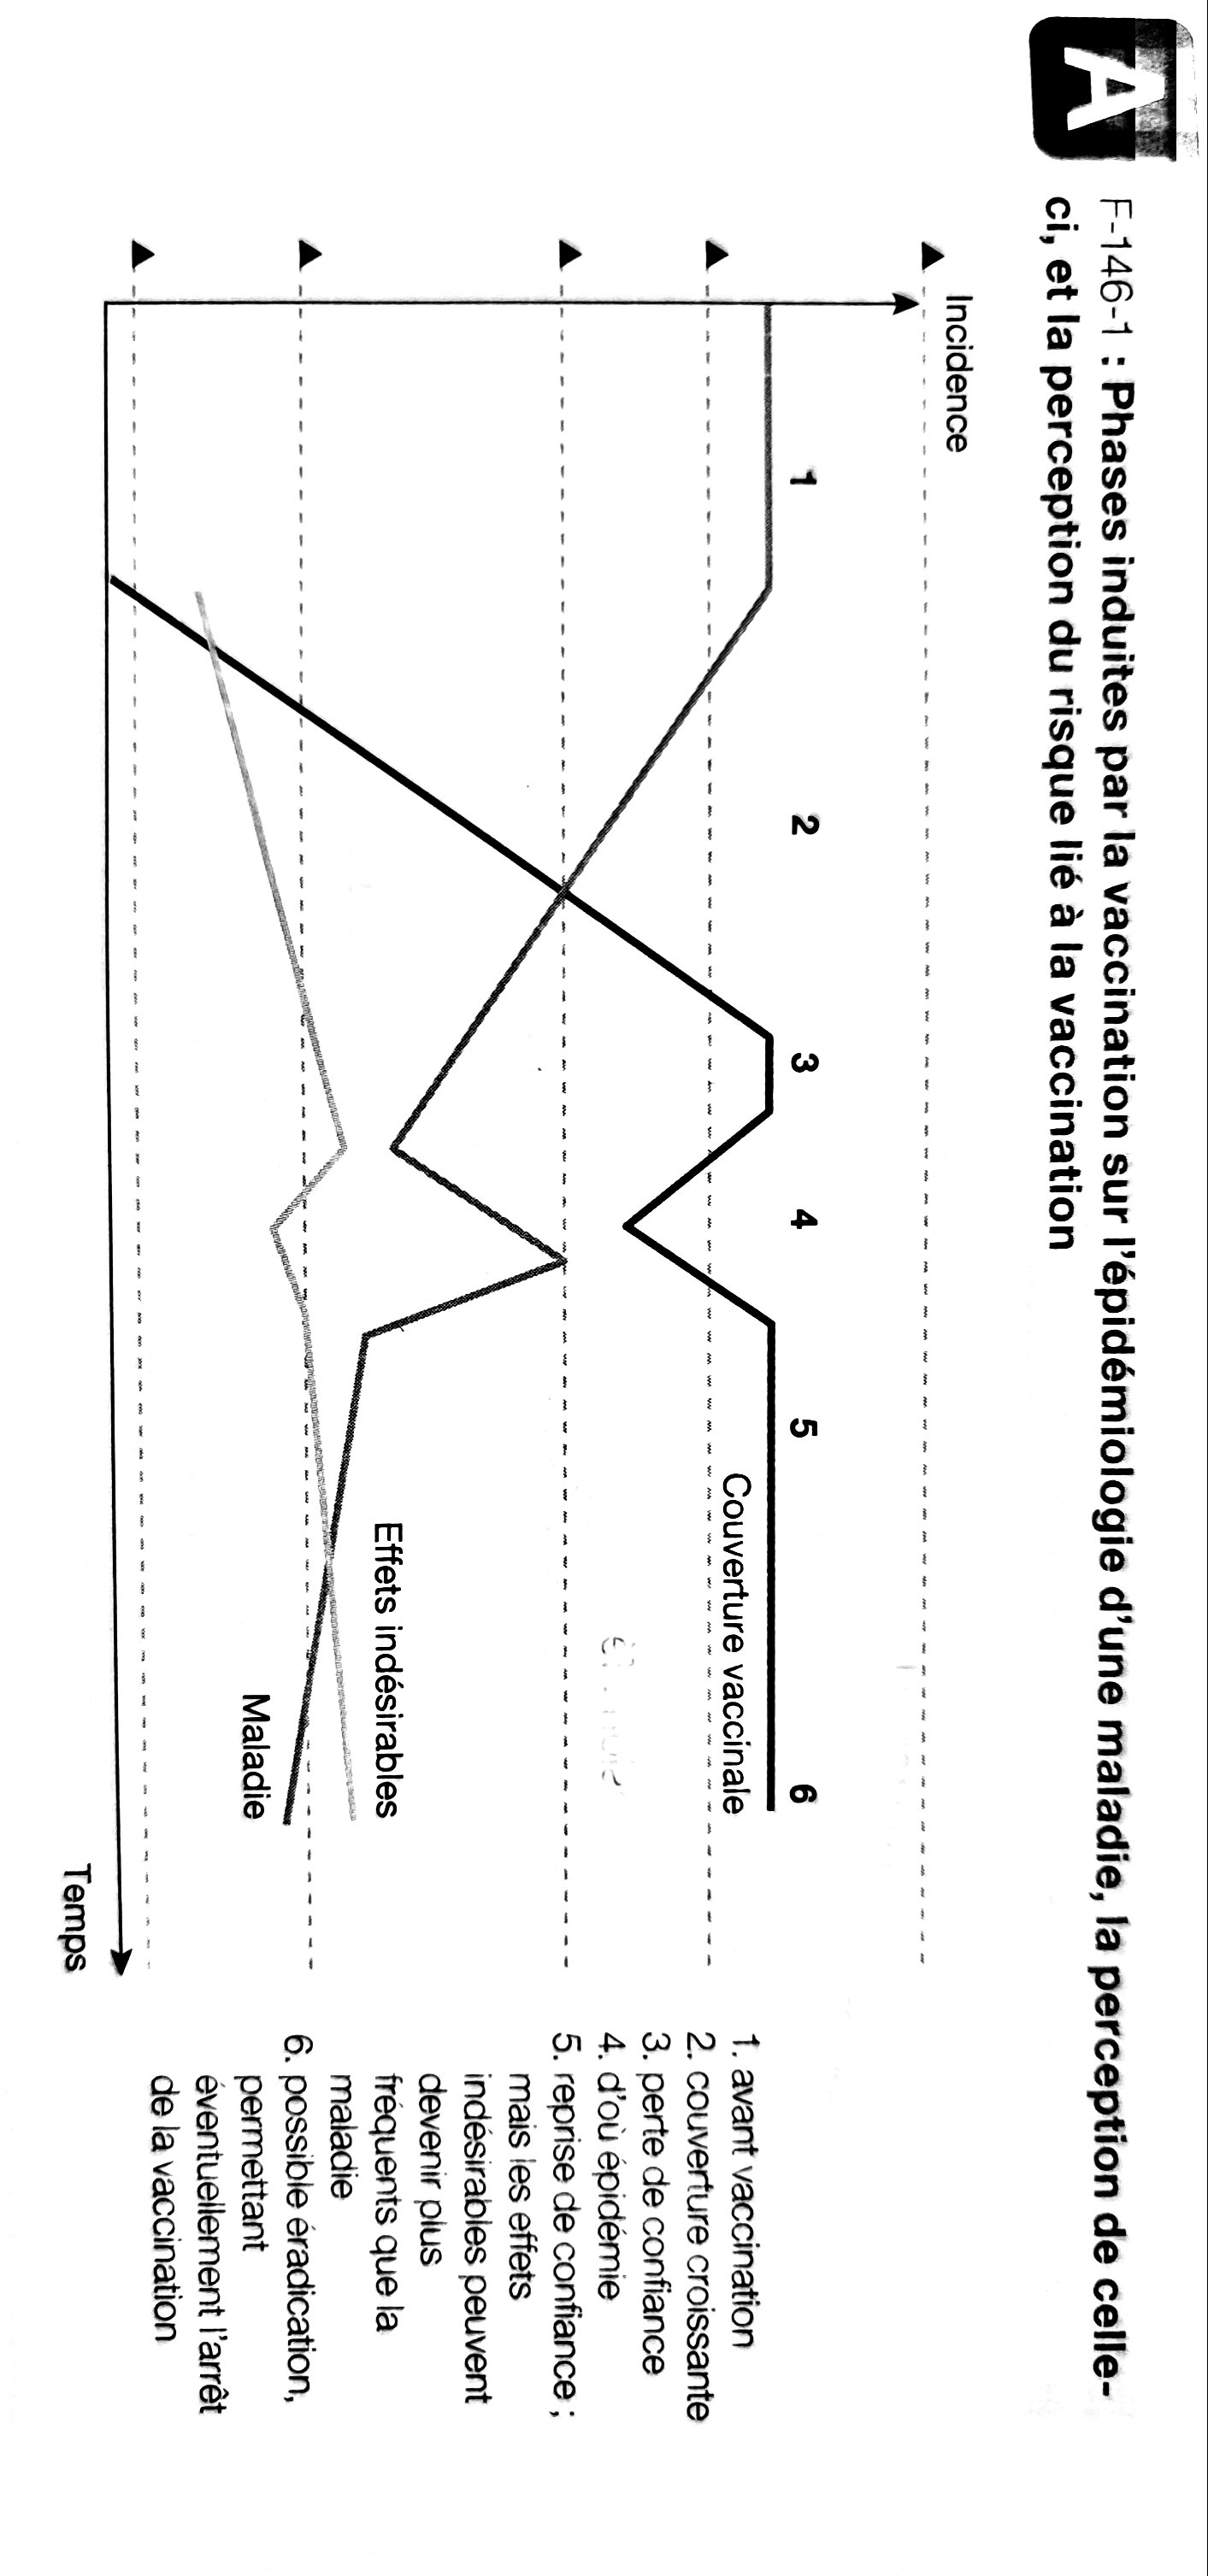
\includegraphics[width=0.5\textwidth, angle=90]{imgs/Perception.jpg} % Pilly 2021 Etudiant CMIT 1st edition
        \end{center}


            Firstly it is an individual protection.

            Secondly it protects the whole population thanks to herd immunity: the pathogen is less likely to be transmitted ; otherwise it would be exponential,
                as people observed for the Covid-19 pandemic.

            % Several study to proove that it is not dangerous for health, especially metal adjuvants 
  
            % three types of population
            % general population, population at-risk (immunodeficient, old people, comorbidities), particularly exposed population (professional, endemic zones)
            % vaccine coverage
            % trips?

            % benefice/risk balance, side effects

        %t. Cinq vaccins sont recommandés pour 
%les personnes de plus de 60 ans : antigrippal, antitétanique, 
%antidiphtérique, anticoquelucheux et antipneumococcique. Par rapport aux s

% avoid disease but also its circulation

%serotherapy

%augmenter les doses d'antigènes 
%pour augmenter la présentation par les cellules dendritiques, utiliser de nouveaux adjuvants pour recruter plus 
%de cellules immunocompétentes (tel que des dérivés de 
%saponine, des liposomes ou des ligands des TLR), varier 
%les voies d'immunisation en privilégiant la voie muqueuse 
%(intra-nasale ou intra-dermique)

        \subsection{New uses and technical challenges}

        
        Currently, there is no real therapeutic vaccines.

        % not only prophylathic but therapeutic

        % prophylatic vaccines VS therapeutic vaccines (avoid expression of the disease)
        % active substance is immunogenic
        % planify vaccines records
        % electronical vaccination record

        % therapeutic, post exposition
        % Hepatitis A for instance, rabies

        %contraindication

    \section{Conclusion}

    % science is not enough
    % rabelais
    % vaccine acceptance is as important as vaccine development

    % what is a vaccine ?

    % a short history : first generation (whole-organism vaccines), second generation (reduce risks from live vaccines = subunit vaccines/toxoid/recombinant),
                        % third generation (RNA/DNA vaccine)
                        %In 2021, Katalin Karikó and Drew Weissman received Columbia University's Horwitz Prize for their pioneering research in mRNA vaccine technology
                        %operatioin warm speed

    % monovalent & polyvalent (more complex : interferences, strength of the immune response)
    % only student monovalent
    % only nanogram or microgram immogen
    % adjuvant (alum) to boost or to store (preservatives, thiomersal/phenoxyethanol, formaldehyde in influenza) -> risk of allergy
    %% excipients also : antibiotics, egg protein, kill 
    % names : abbreviation

    % legislation
    % patent : stakes : licensing
    % vaccine acceptance by population (save live, economic)
    % manufacturing, distribution, losgitical factor : prioritize
    % state role and WHO role
    % record for adverse eeffects...
    % EMA/FDA



    % which phase for a vaccine development
    %scientific and then safety 
    % use and scheduling ? many vaccine when young, need combination of injections
    % different  phases
    % paradox of economic development of vaccines : role of government, universities and non-profit organizations
    % need infrastructure and workforce
    % The large number of vaccines and boosters recommended (up to 24 injections by age two) has led to problems with achieving full compliance.
    % to healthy people : huge quality needed
    % build : bioreactor
    % vials = flacons
    % filling vials : difficult step

    % key players & firms
    % 10/15 years official development
    % from injection to oral vaccines (ouverture)

    % link to veterinary medicine

    % revoir test ELISA principe
    % next stakes : vaccine resistance (same as antimicrobial resistance) (immune evasion) -> covid, this is the case, if total protection less likely than only against serious forms
    % transgenic plant
    

    %https://biontech.de/covid-19-portal/mrna-vaccines (interesting schema)
    %https://sitn.hms.harvard.edu/flash/2015/rna-vaccines-a-novel-technology-to-prevent-and-treat-disease/
    % Bill & Melinda Gates Foundation invested $53 million in the German company, CureVac, which specializes in the development of these vaccines
    % perspective for the future as regard influenza vaccines : influenza vaccine, whereas the company CureVac claims that RNA-based vaccines could be manufactured in less than two months at a lower production cost, (harvard) + cancer vaccines
    %

    \newpage
    
    \nocite{*}
    \printbibliography

    \newpage

    \appendix

    \section {Source code}
        The source code of this document is available at \url{https://github.com/florian6973/biology-report}.
        It was written using Visual Studio Code and compiled with TeX Live (Windows).

        In this repository a beamer is also available, to present this report.

\end{document}